% CoopNS-OCT Overall Architecture — v7 final: all labels clear
\documentclass[border=3pt]{standalone}
\usepackage{tikz}
\usepackage{amsmath,amssymb}
\usetikzlibrary{arrows.meta,positioning,fit,backgrounds,calc,decorations.pathreplacing}

\begin{document}
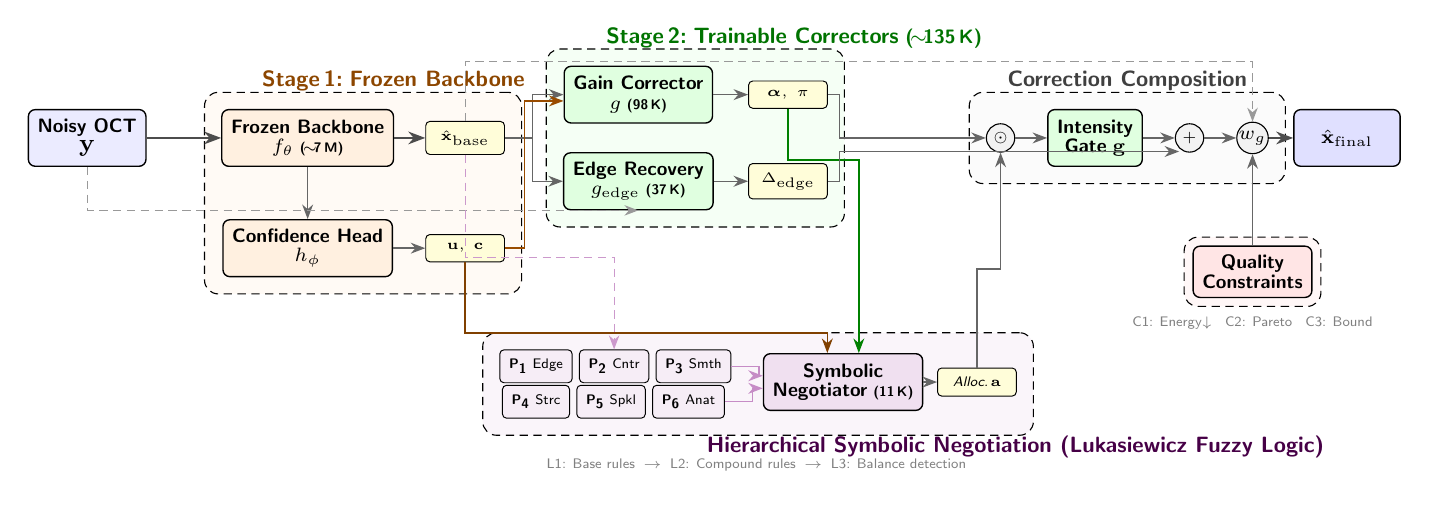
\begin{tikzpicture}[
    >=Stealth,
    inout/.style={draw, rounded corners=2.5pt, fill=blue!8, minimum height=0.72cm, minimum width=1.35cm, font=\sffamily\scriptsize\bfseries, align=center, line width=0.5pt},
    frozenblk/.style={draw, rounded corners=2.5pt, fill=orange!12, minimum height=0.72cm, minimum width=1.7cm, font=\sffamily\scriptsize\bfseries, align=center, line width=0.5pt},
    corrblk/.style={draw, rounded corners=2.5pt, fill=green!12, minimum height=0.72cm, minimum width=1.55cm, font=\sffamily\scriptsize\bfseries, align=center, line width=0.5pt},
    symbblk/.style={draw, rounded corners=2.5pt, fill=violet!12, minimum height=0.72cm, minimum width=1.55cm, font=\sffamily\scriptsize\bfseries, align=center, line width=0.5pt},
    predblk/.style={draw, rounded corners=1.5pt, fill=violet!7, minimum height=0.3cm, minimum width=0.8cm, font=\sffamily\tiny, align=center, line width=0.35pt},
    constblk/.style={draw, rounded corners=2.5pt, fill=red!10, minimum height=0.65cm, minimum width=1.35cm, font=\sffamily\scriptsize\bfseries, align=center, line width=0.5pt},
    mapblk/.style={draw, rounded corners=1.5pt, fill=yellow!15, minimum height=0.34cm, minimum width=1.0cm, font=\sffamily\tiny\itshape, align=center, line width=0.35pt},
    opcirc/.style={draw, circle, fill=gray!10, minimum size=0.36cm, font=\sffamily\tiny\bfseries, inner sep=0pt, line width=0.4pt},
    arr/.style={->, line width=0.5pt, color=black!60},
    arrbold/.style={->, line width=0.7pt, color=black!70},
    arrdash/.style={->, line width=0.45pt, color=black!40, densely dashed},
    lbl/.style={font=\sffamily\tiny\color{black!50}, align=center},
    glbl/.style={font=\sffamily\tiny\bfseries},
    gbox/.style={draw, densely dashed, rounded corners=5pt, line width=0.4pt, inner sep=6pt},
]

% =====================================================================
% COLUMN 1: Input
% =====================================================================
\node[inout] (input) at (0, 0) {Noisy OCT\\[-1pt]{\small$\mathbf{y}$}};

% =====================================================================
% COLUMN 2: Frozen Backbone
% =====================================================================
\node[frozenblk] (bbone) at (2.8, 0) {Frozen Backbone\\[-1pt]$f_\theta$\;{\tiny($\!\sim\!$7\,M)}};
\node[frozenblk] (conf) at (2.8, -1.4) {Confidence Head\\[-1pt]$h_\phi$};
\node[mapblk] (xbase) at (4.8, 0) {$\hat{\mathbf{x}}_{\mathrm{base}}$};
\node[mapblk] (uc) at (4.8, -1.4) {$\mathbf{u},\;\mathbf{c}$};

\draw[arrbold] (input) -- (bbone);
\draw[arrbold] (bbone) -- (xbase);
\draw[arr] (bbone) -- (conf);
\draw[arr] (conf) -- (uc);

% =====================================================================
% COLUMN 3 upper: Corrector Modules
% =====================================================================
\node[corrblk] (gain) at (7.0, 0.55) {Gain Corrector\\[-1pt]$g$\;{\tiny(98\,K)}};
\node[corrblk] (edge) at (7.0, -0.55) {Edge Recovery\\[-1pt]$g_{\mathrm{edge}}$\;{\tiny(37\,K)}};
\node[mapblk] (gainout) at (8.9, 0.55) {$\boldsymbol{\alpha},\;\pi$};
\node[mapblk] (edgeout) at (8.9, -0.55) {$\Delta_{\mathrm{edge}}$};

\draw[arr] (xbase.east) -- ++(0.35cm,0) coordinate (xfan) |- (gain.west);
\draw[arr] (xfan) |- (edge.west);
\draw[arrdash] (input.south) -- ++(0,-0.55cm) -| ([xshift=-0.2cm]edge.south) -- (edge.south);
\draw[arr, color=orange!60!black] (uc.east) -- ++(0.25cm,0) |- ([yshift=-0.08cm]gain.west);
\draw[arr] (gain) -- (gainout);
\draw[arr] (edge) -- (edgeout);

% =====================================================================
% COLUMN 3 lower: Predicates + Symbolic Negotiator
% =====================================================================
\node[predblk] (p1) at (5.7, -2.9) {\textbf{P\textsubscript{1}} Edge};
\node[predblk, right=0.08cm of p1] (p2) {\textbf{P\textsubscript{2}} Cntr};
\node[predblk, right=0.08cm of p2] (p3) {\textbf{P\textsubscript{3}} Smth};
\node[predblk] (p4) at (5.7, -3.35) {\textbf{P\textsubscript{4}} Strc};
\node[predblk, right=0.08cm of p4] (p5) {\textbf{P\textsubscript{5}} Spkl};
\node[predblk, right=0.08cm of p5] (p6) {\textbf{P\textsubscript{6}} Anat};

\draw[arrdash, color=violet!40] (xbase.south) -- ++(0,-1.3cm) -| (p2.north);

\node[symbblk] (negot) at (9.6, -3.1) {Symbolic\\[-1pt]Negotiator\;{\tiny(11\,K)}};

\draw[arr, color=violet!45] (p3.east) -- ++(0.35cm,0) |- ([yshift=0.08cm]negot.west);
\draw[arr, color=violet!45] (p6.east) -- ++(0.35cm,0) |- ([yshift=-0.08cm]negot.west);

\draw[arr, color=green!50!black] (gainout.south) -- ++(0,-0.65cm) -| ([xshift=0.2cm]negot.north);
\draw[arr, color=orange!50!black] (uc.south) -- ++(0,-0.9cm) -| ([xshift=-0.2cm]negot.north);

\node[mapblk] (alloc) at (11.3, -3.1) {Alloc.\,$\mathbf{a}$};
\draw[arr] (negot) -- (alloc);

% Level annotation — placed BELOW the group box
\node[lbl] (lvlannot) at (8.5, -4.15) {L1: Base rules\;\;$\rightarrow$\;\;L2: Compound rules\;\;$\rightarrow$\;\;L3: Balance detection};

% =====================================================================
% COLUMN 4: Correction Composition
% =====================================================================
\node[opcirc] (odot) at (11.6, 0) {$\odot$};
\node[corrblk, minimum width=1.2cm] (igate) at (12.8, 0) {Intensity\\[-1pt]Gate\;$\mathbf{g}$};
\node[opcirc] (plus) at (14.0, 0) {$+$};
\node[opcirc, minimum size=0.4cm] (wg) at (14.8, 0) {\scriptsize$w_g$};
\node[inout, fill=blue!12] (final) at (16.0, 0) {$\hat{\mathbf{x}}_{\mathrm{final}}$};

\draw[arr] (gainout.east) -- ++(0.15cm,0) |- (odot.west);
\draw[arr] (alloc.north) -- ++(0,1.25cm) -| (odot.south);
\draw[arr] (odot) -- (igate);
\draw[arr] (igate) -- (plus);
\draw[arr] (plus) -- (wg);
\draw[arrbold] (wg) -- (final);
\draw[arr] (edgeout.east) -- ++(0.15cm,0) |- ([yshift=-0.04cm]plus.south west);
\draw[arrdash] (xbase.north) -- ++(0,0.75cm) -| (wg.north);

% Quality Constraints
\node[constblk] (qconst) at (14.8, -1.7) {Quality\\[-1pt]Constraints};
\draw[arr] (qconst) -- (wg);
\node[lbl, below=0.12cm of qconst] {C1: Energy$\downarrow$\;\; C2: Pareto\;\; C3: Bound};

% =====================================================================
% GROUP BOXES
% =====================================================================
\begin{scope}[on background layer]
    % Stage 1
    \node[gbox, fill=orange!4,
          fit=(bbone)(conf)(xbase)(uc),
          label={[glbl, color=orange!55!black, anchor=south west, inner sep=0pt]above left:{\sffamily\footnotesize Stage\,1:\;Frozen Backbone}}] {};

    % Stage 2
    \node[gbox, fill=green!4,
          fit=(gain)(edge)(gainout)(edgeout),
          label={[glbl, color=green!45!black, anchor=south west, inner sep=0pt]above left:{\sffamily\footnotesize Stage\,2:\;Trainable Correctors\;{\scriptsize($\!\sim\!$135\,K)}}}] {};

    % Symbolic negotiation — label at BOTTOM LEFT to avoid collision
    \node[gbox, fill=violet!4,
          fit=(p1)(p4)(p6)(negot)(alloc),
          label={[glbl, color=violet!55!black, anchor=north west, inner sep=0pt]below left:{\sffamily\footnotesize Hierarchical Symbolic Negotiation (Lukasiewicz Fuzzy Logic)}}] {};

    % Correction composition
    \node[gbox, fill=gray!3,
          fit=(odot)(igate)(plus)(wg),
          label={[glbl, color=gray!50!black, anchor=south, inner sep=0pt]above:{\sffamily\footnotesize Correction Composition}}] {};

    % Quality constraints
    \node[gbox, fill=red!3, fit=(qconst), inner sep=3pt] {};
\end{scope}

\end{tikzpicture}
\end{document}
